\documentclass[10pt]{article}\usepackage[margin=.65in]{geometry}\usepackage{graphicx,longtable,array,hyperref}\begin{document}
\section*{Reviewed branch components: additive overview}
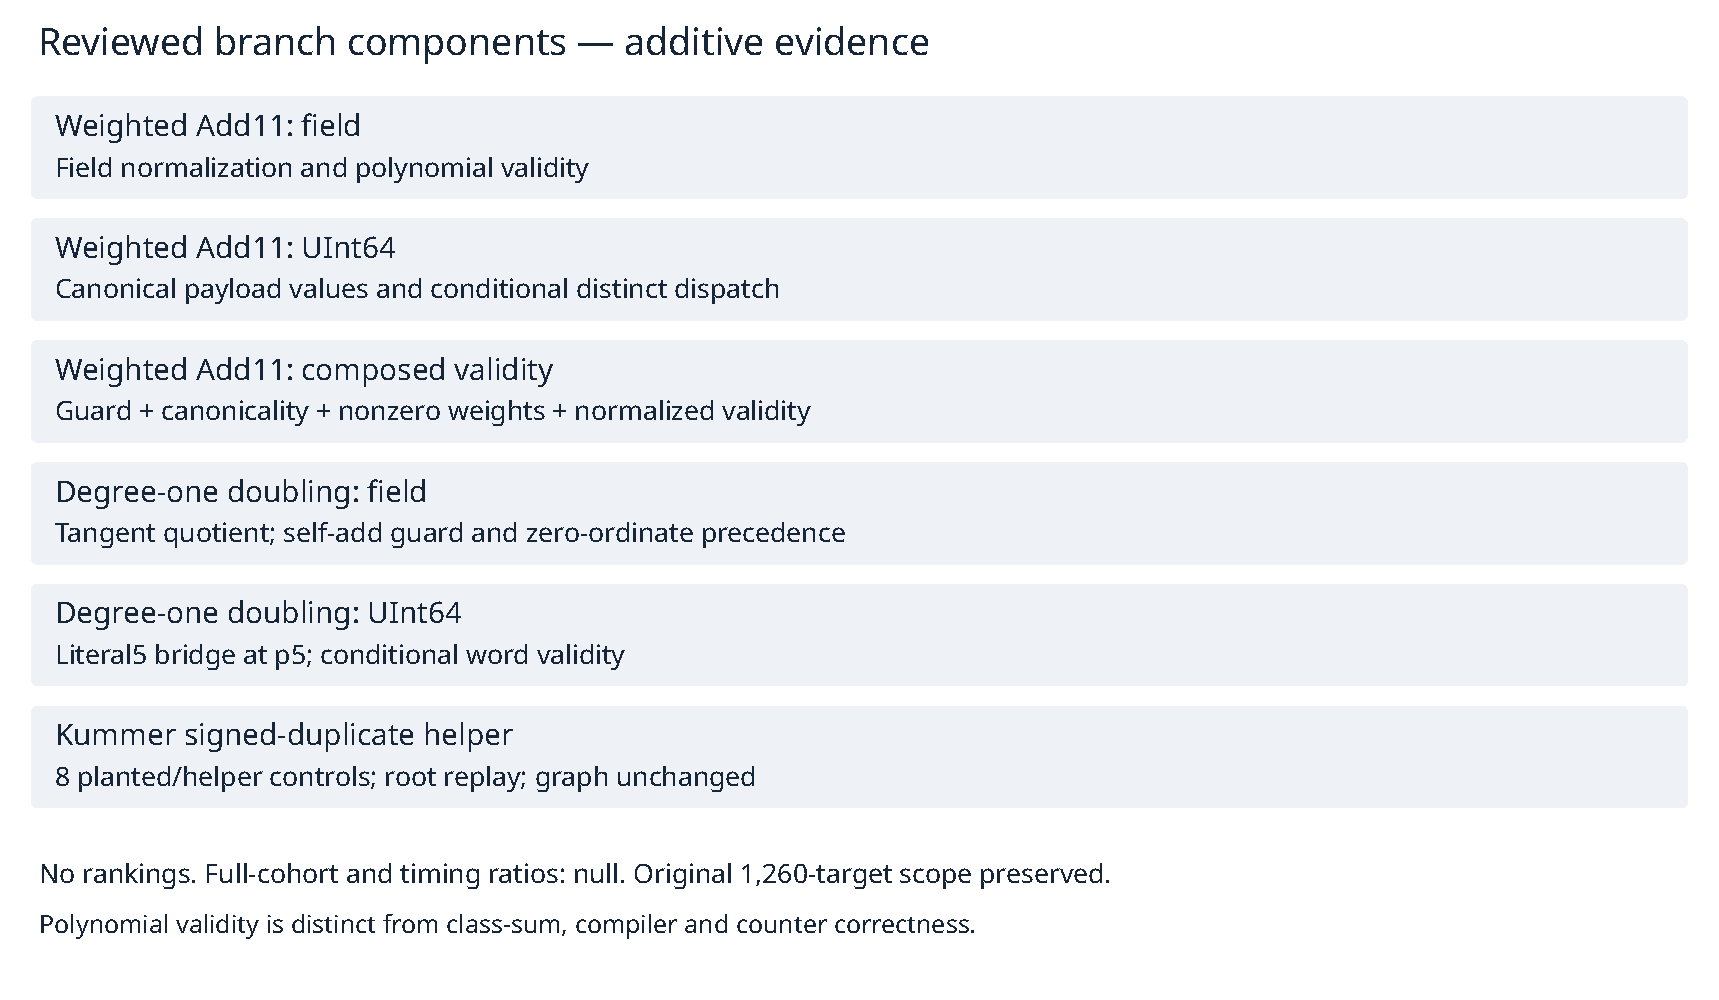
\includegraphics[width=\linewidth]{overview.pdf}
\noindent This report indexes reviewed local constructions and fixed software controls. It introduces no new cohort observations, rankings or cost comparisons. All new full-cohort and timing-ratio fields are null. Native proof/check counts describe validation, not performance.
\paragraph{Evidence access} INDEX.md and index.json contain relative links to producer reports and independent reviews, with exact SHA256 bindings. Their intended publication directory is \texttt{report-branch-completion}; the full relative base is recorded in index.json. Previous reports remain unchanged.
\paragraph{Software snapshot} The historical full-library result remains 5,792 passed, one failed and 128 ignored, with a passing isolated replay. Further software checks remain pending in the retained snapshot; this report makes no new current aggregate-test assertion. Native receipts are linked separately.
\newpage
\section*{Assumptions and review boundaries}
\begin{longtable}{p{.25\linewidth}p{.69\linewidth}}
\textbf{Component}&\textbf{Conditions and limits}\\\hline
Weighted Add11 field & Four nonzero weights, distinct normalized x and both input divisibilities over a common polynomial. Field normalization and polynomial validity; no class-sum claim.\\[7pt]
Weighted Add11 word & Prime $5\le p<2^{31}$ and eight canonical input words. Exact exponent-five value model and six decoded coordinates. Field n=1, no tables and normal counter execution are source conditions; compiler/counting not proved.\\[7pt]
Add11 composed validity & Previous bounds plus nonzero word weights and input validity. Conclusion includes distinct dispatch. The nonunit F7 control uses $f=X^2$ and is not a smooth genus-two fixture.\\[7pt]
Doubling field & Monic quintic with zero $X^4$ coefficient, nonzero z,w,y,2 and point equation. Derivative may vanish. Self-add guard only; nonsingularity is unnecessary for polynomial divisibility but separate for geometric interpretation.\\[7pt]
Doubling word & Four canonical coefficients and four canonical coordinates. Literal5 reduction covers p5. Decoded nonzero assumptions and point equation yield normalized validity. The p5 $X^5+1$ control is nonsmooth; normal-curve preprocessing is not proved.\\[7pt]
Kummer duplicate helper & Eight native controls reproduced independently by root. Two informative candidates are deliberately planted using known k and verified in the Jacobian. Each graph snapshot remains one edge/zero cycles. Valid labels, target identity, membership Q in generated subgroup and eligibility remain caller requirements. No new trajectory or natural collision yield.\\
\end{longtable}
\section*{Original completion criteria remain intact}
The four-lead inventory remains: factor-base/graph sweep, published weighted genus-two law, point-driven pencil, and sign-safe Kummer walk. Historical completed cohorts stay separate from these new local checks. Additional graph policies require prospective arms; unproved law branches and geometric/compiled correspondence remain explicit; the pencil retains its full 1,260-target requirement and all missing/capped outcomes; Kummer fixture families are not pooled.

The five followup obligations remain word correspondence, collector invariants, exceptional branches, Kummer transitions and target-information/source-row correspondence. Local branch completion does not close the whole walk or collector.

All original target identities, control arms, complete accounting, qualified timing and independent review requirements are preserved. The separate18-slot upper gate is not enrolled cohort coverage. No resource authorization, deadline or prior charge is reset; no scientific execution is authorized by this report.
\end{document}